\chapter{Introducción}
    
\lhead{Capítulo 1 \emph{Introducción}}

    \par En el vertiginoso mundo de la tecnología de drones, la seguridad y la eficiencia de las operaciones son imperativos clave para su integración exitosa en diversas aplicaciones, desde la entrega de paquetes hasta la inspección de infraestructuras críticas. La navegación segura y autónoma de drones, especialmente en entornos complejos y cambiantes, representa un desafío crucial que ha impulsado la investigación y el desarrollo de algoritmos avanzados. Este trabajo se centra en un aspecto fundamental de esta problemática: la evasión de obstáculos.

\section{Resumen de los antecedentes}

    \par En la literatura existe una amplia gama de técnicas y métodos para abordar el problema de la evasión de obstáculos para drones. 
    
    \par Métodos basados en aprendizaje por reforzamiento (del inglés \textit{reinforcement leanring}) tales como los empleados en \cite{Tu2023} y en \cite{Xue2021} han probado ser efectivos en el entrenamiento de políticas reactivas de evasión de obstáculos. Estas políticas, a partir de entradas sensoriales en forma de imágenes producidas por cámaras \textit{RGB} o de profundidad, producen trayectorias sin colisiones definidas por un espacio de acciones, todo esto sin tener información directa acerca de la localización de los obstáculos en el espacio. Estos métodos requieren un proceso de entrenamiento complejo tal como se puede observar en la Figura \ref{fig:rl-training-process}. Adicionalmente, estos métodos introducen latencia al momento de realizar inferencia debido a la complejidad de los modelos (usualmente requiriendo múltiples redes neuronales para su funcionamiento), lo cual hace que estos métodos no sean ideales para drones con capacidad de procesamiento limitada. Adicionalmente la definición del espacio de acciones es una tarea complicada y puede resultar en trayectorias difíciles de ejecutar.

    \begin{figure}[H]
        \centering
        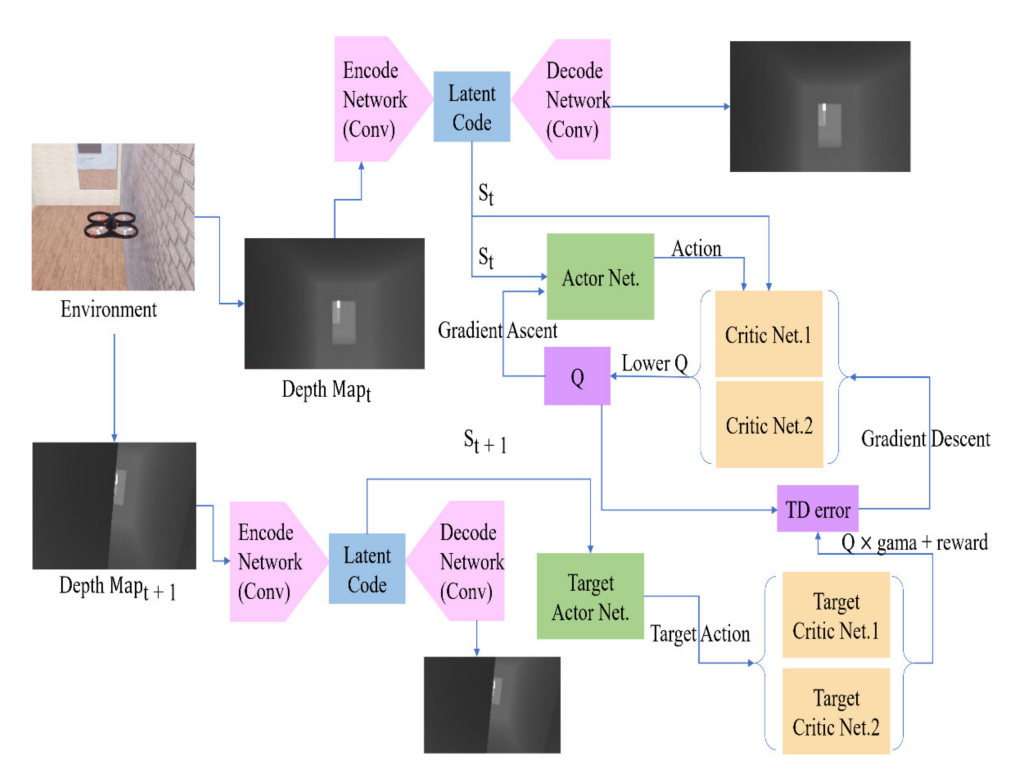
\includegraphics[scale=0.4]{partes/img/RL-training-process.png}
        \caption[Diagrama de flujo del proceso de entrenamiento utilizado en \textit{Vision Based Drone Obstacle Avoidance by Deep Reinforcement Learning}]{Diagrama de flujo del proceso de entrenamiento utilizado en \cite{Xue2021}.}
        \label{fig:rl-training-process}
    \end{figure}

    \par Métodos con información parcial del entorno tales como el propuesto en \cite{Zhang2019} utilizan la información conocida del entorno para planear trayectorias libres de colisión antes de la ejecución del vuelo (proceso denominado \textit{trajectory planning} o planeamiento de trayectorias), reduciendo la carga computacional del algoritmo durante la ejecución de la trayectoria, permitiendo que los recursos computacionales del dron estén disponibles para otras tareas. En particular, el método propuesto en \cite{Zhang2019}, genera una colección de trayectorias libres de colisión, y alterna entre las distintas trayectorias o \textit{lanes} al momento de ejecución, dependiendo de la información de los obstáculos observados, dándole la capacidad al dron de reaccionar a obstáculos no provistos en la información inicial del entorno. Sin embargo, el requerimiento de poseer información previa sobre el entorno hace que sea complicado que este método opere en entornos genéricos o desconocidos.

    \par Otros métodos utilizan redes neuronales convolucionales (\textit{CNN} del inglés \textit{convolutional neural networks}) para directa o indirectamente producir trayectorias libres de colisión en entornos desconocidos. En el método propuesto en \cite{Yang2021} se utiliza una \textit{CNN} probabilística, que a partir de una cámara monocular genera mapas de profundidad y mapas de confianza probabilísticos, que posteriormente son utilizados para navegar arbitrariamente el entorno sin generar colisiones. Sin embargo, las trayectorias generadas no van dirigidas hacia ningún objetivo en particular, lo cual hace que sea de poca utilidad en la práctica.

    \par Los métodos que utilizan \textit{CNN} requieren una base de datos para su proceso de entrenamiento. Esto limita la gama de tareas que puede resolver una \textit{CNN} a las tareas para las cuales existe una base datos disponible, por ejemplo, se puede entrenar una \textit{CNN} para estimar imágenes de profundidad a partir de imágenes \textit{RGB} utilizando bases de datos como \textit{KITTI} \cite{Geiger2013} y \textit{TUM RGB-D} \cite{Sturm2012}. Las \textit{CNN} tienen la ventaja de que son relativamente sencillas de entrenar con respecto a otras alternativas (como el aprendizaje por reforzamiento), por lo cual resultan atractivas para resolver problemáticas en donde se tiene disponible una base de datos. Es importante destacar que actualmente no hay bases de datos generales enfocadas en la tarea de la evasión de obstáculos para drones, limitando el uso que se le puede dar a las \textit{CNN} dentro de esta problemática. 
    
    \par En el método propuesto por Loquercio et al. (2021) \cite{Loquercio2021} se soluciona el requerimiento de poseer una base de datos para el entrenamiento de una \textit{CNN} como política de evasión de obstáculos; empleando el denominado entrenamiento por imitación (del inglés \textit{imitation learning}), en lugar de aplicar entrenamiento supervisado sobre una base de datos ya existente, se utiliza, dentro de un entorno de simulación, una política experta con acceso privilegiado a la información de los obstáculos del entorno (el ``experto'') para generar una base de datos de trayectorias libres de colisión. Esta base de datos contiene ejemplos de trayectorias libres de colisión dado una imagen de profundidad, mediciones inerciales del estado del dron y la dirección hacia donde se encuentra el objetivo del dron. Esto permite entrenar una política ``estudiante'' (modelada como una \textit{CNN}) de generación de trayectorias directa a partir de imágenes de profundidad, mediciones inerciales y una dirección objetivo. Una visión general del metodo se puede observar en la Figura \ref{fig:agile-autonomy-overview}.

    \begin{figure}[H]
        \centering
        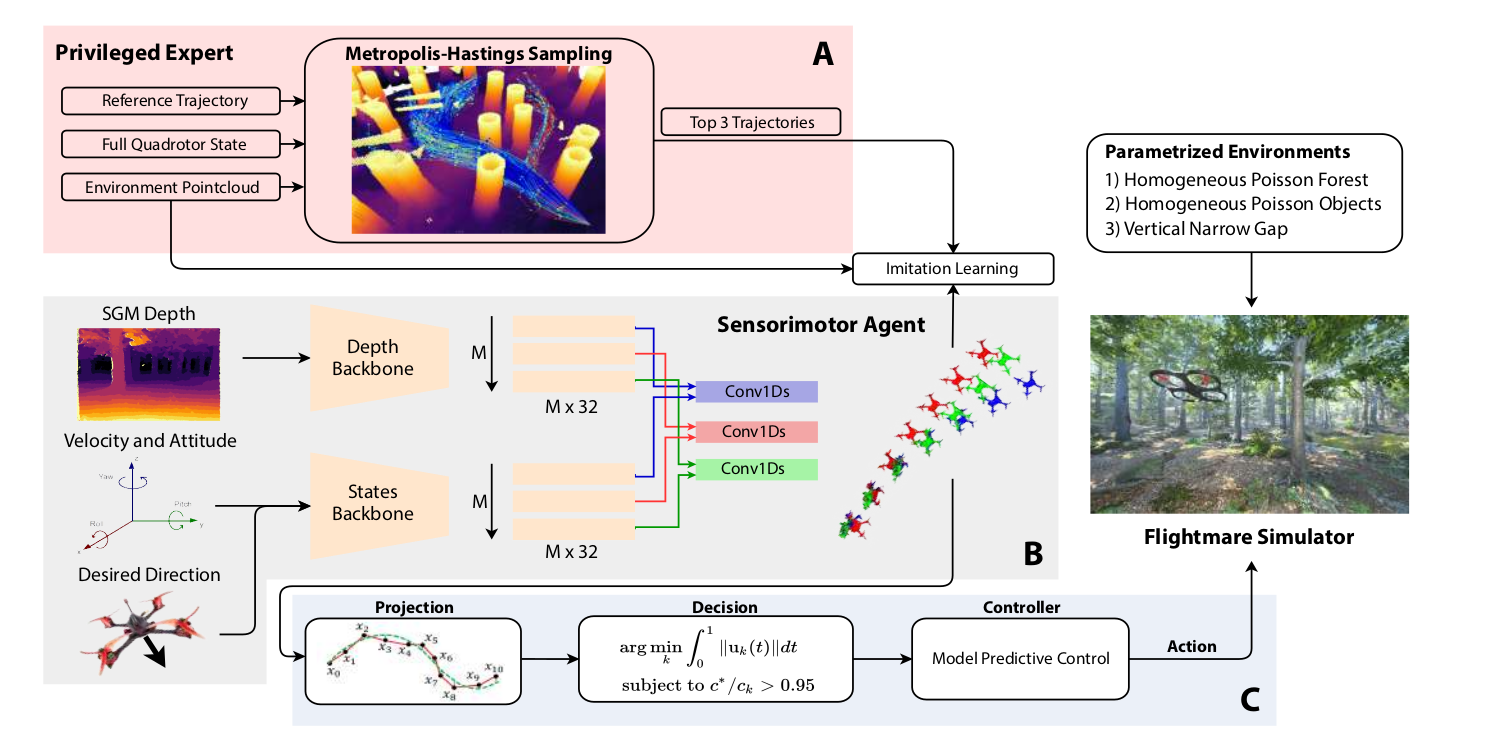
\includegraphics[scale=0.3]{partes/img/agile-autonomy-overview.png}
        \caption[Visión general del método del método utilizado en \textit{Learning high-speed flight in the wild}]{Visión general del método utilizado en \cite{Loquercio2021}. \textbf{(A)} El ``experto'' genera una distribución de trayectorias libre de colisión que siguen una trayectoria de referencia. Las trayectorias generadas están condicionadas por la completa información de obstáculos del entorno. \textbf{(B)} La política ``estudiante'' es entrenada mediante entrenamiento por imitación para predecir las mejores 3 trayectorias a partir una estimación de la profundidad, mediciones inerciales del dron y una dirección objetivo. \textbf{(C)} Las predicciones son proyectadas en el espacio de las trayectorias polinomiales y finalmente la trayectoria con el costo de predicción mas bajo es ejecutada por el modelo de control. }
        \label{fig:agile-autonomy-overview}
    \end{figure}
    
    La política ``estudiante'' puede transferirse trivialmente a un ambiente fuera de simulación, siempre y cuando al momento de generar la base datos de entrenamiento se utilicen métodos de estimación de imágenes de profundidad cuya salida posea niveles similares de ruido tanto en simulación como en entornos reales, tales como \textit{SGM} \cite{Hirschmüller2007} (del inglés \textit{semi global matching}). Finalmente, el modelo propuesto en \cite{Loquercio2021} resulta bastante conveniente para la evasión de obstáculos pues, es sencillo de entrenar, la política ``estudiante'' se modela utilizando una \textit{CNN} ligera \cite{Howard2019} que no introduce demasiada latencia al momento de ejecución, no necesita información previa del entorno, es fácil de transferir para funcionamiento en ambientes fuera de simulación y toma en cuenta la dirección de objetivo del dron, lo cual produce trayectorias libres de colisión que se dirigen al objetivo.

\section{Justificación y planteamiento del problema}

    \par Los drones han experimentado un crecimiento exponencial en su adopción en diversas aplicaciones, desde la agricultura de precisión hasta la logística de entrega y la vigilancia. Sin embargo, uno de los desafíos fundamentales que enfrentan los drones es su capacidad para operar de manera segura y autónoma en entornos dinámicos y desconocidos, donde los obstáculos pueden surgir en cualquier momento y lugar. La evasión de obstáculos es esencial para garantizar la seguridad de las operaciones de los drones y su capacidad de navegación autónoma en entornos complejos.

    \par En este contexto, el presente trabajo se centra en la implementación de un algoritmo de evasión de obstáculos para drones, específicamente diseñado para abordar la falta de información a priori sobre la ubicación de los obstáculos. Este enfoque reactivo permitirá que los drones tomen decisiones en tiempo real para evitar obstáculos de manera segura y eficiente, lo que es esencial para su aplicación en entornos urbanos, industriales y otros escenarios realistas.

    \par La empresa ACSL (del inglés \textit{Autonomous Control Systems Laboratory}), con sede en Japón, se ha destacado como líder en la investigación y desarrollo de soluciones de control autónomo para drones. ACSL ha identificado la necesidad crítica de mejorar la capacidad de los drones para evadir obstáculos de manera efectiva, lo que impulsará la seguridad de las operaciones y abrirá nuevas oportunidades de aplicación en una variedad de industrias.

    \par La implementación exitosa de un algoritmo de evasión de obstáculos reactivo tiene el potencial de revolucionar la seguridad y la autonomía de los drones, lo que beneficiaría a una amplia gama de industrias, desde la entrega de paquetes hasta la inspección de infraestructuras críticas. Además, contribuirá al liderazgo continuo de ACSL en el campo de la tecnología de drones, consolidando su posición como un actor clave en la innovación y desarrollo de soluciones de vanguardia en Japón y a nivel internacional.
        
   
\section{Objetivos}

    \subsection{Objetivo general}
    
    Implementar un algoritmo de evitación de obstáculos para drones autónomos y realizar
    pruebas de dicha implementación tanto en entorno de simulación como en el campo.
    
    \subsection{Objetivos específicos}
    
    \begin{itemize}
        \item Investigar el estado del arte de los algoritmos de evitación de obstáculos para drones autónomos.
        \item Implementar un algoritmo de evitación de obstáculos para drones autónomos sobre un ambiente de simulación y realizar pruebas en dicho ambiente.
        \item Ajustar la implementación del algoritmo seleccionado al hardware de un dron autónomo realizando las optimizaciones necesarias y realizar pruebas de campo de dicha implementación.
    \end{itemize}

\section{Estructura del trabajo}

    \par Este trabajo se encuentra dividido en seis capítulos de la siguiente manera:
    
    \par El \textbf{Capítulo 2} describe la empresa receptora en donde se realizó este trabajo, el Laboratorio de Sistemas de Control Autónomo (ACSL, del inglés \textit{Autonomous Control Systems Laboratory}), localizado en Tokio, Japón. 
    
    \par En el \textbf{Capítulo 3} se explican las bases teóricas de los principales algoritmos utilizados en este trabajo. 
    
    \par El \textbf{Capítulo 4} incluye la revisión del estado del arte sobre los métodos de evasión de obstáculos para drones autónomos. 
 
    \par El \textbf{Capítulo 5} muestra la implementación del algoritmo de evitación de obstáculos y la arquitectura utilizada.
    
    \par En el \textbf{Capítulo 6} se muestran y se discuten los resultados obtenidos.
    
    \par Finalmente en el \textbf{Capítulo 7} se presentan las conclusiones del presente trabajo, así como las recomendaciones para posibles trabajos futuros. 
